\documentclass[11pt,a4paper]{article}
\usepackage[margin=27mm]{geometry}
\usepackage{amsmath,amssymb,amsthm,mathtools,booktabs,graphicx,xurl,hyperref}
\emergencystretch=2em
\hypersetup{colorlinks=true,linkcolor=black,citecolor=black,urlcolor=blue}
\newtheorem{theorem}{Theorem}[section]
\newtheorem{proposition}[theorem]{Proposition}
\newtheorem{corollary}[theorem]{Corollary}
\newtheorem{lemma}[theorem]{Lemma}
\theoremstyle{definition}\newtheorem{definition}[theorem]{Definition}
\theoremstyle{remark}\newtheorem{remark}[theorem]{Remark}
\newcommand{\Tr}{\operatorname{Tr}}
\newcommand{\diag}{\operatorname{diag}}
\newcommand{\ket}[1]{\lvert #1\rangle}
\newcommand{\bra}[1]{\langle #1\rvert}
\newcommand{\op}{\mathrm{op}}
\newcommand{\one}{\mathbf{1}}
\newcommand{\E}{\mathcal E}
\newcommand{\F}{\mathcal F}
\newcommand{\R}{\mathcal R}
\newcommand{\J}{\mathcal J}
\title{Negative mutual information in time\\in the smallest dimensions}
\author{Anonymous}
\date{15 November 2026\\[2pt]\small Version 0.1.0-candidate, DOI \href{https://doi.org/10.5281/zenodo.24269629}{10.5281/zenodo.24269629}}
\begin{document}
\maketitle

\begin{abstract}
Fullwood and Parzygnat proposed a mutual information between the input and the output of a quantum process, built from the signed entropy $S(X)=-\Tr(X\log|X|)$ of the process's quantum state over time (pseudo-density matrix). They conjectured that it is never negative. Fullwood and Yang proved the conjecture when the input is a qubit, and a public five-dimensional Werner--Holevo example has since shown that it fails in general. This paper determines exactly where it starts to fail. A violation needs an input of dimension at least three, an output of dimension at least two and an initial state of rank at least two, and one explicit process attains all three bounds at once: a qutrit-to-qubit channel acting on a rank-two state, certified by exact root isolation and interval arithmetic. A second, qutrit-to-qutrit family explains the mechanism. It is a coherent completion of a qubit erasure channel. Its spectrum is explicit, and at $t=5/21$ its negativity reduces to the integer inequality $2573571875<8707129344$. Along the family the mutual information is strictly convex, and it is negative exactly on the interval $0<t<(\sqrt{33}-1)/16$. The violations persist for full-rank states and channels with positive-definite Choi matrix. A short structural lemma shows why coherence is essential: when a channel has no coherence between the support of a rank-two state and its complement, the mutual information equals that of a qubit-input process and is therefore non-negative. Comparing coherent and incoherent completions of the same erasure channel gives processes that agree on the occupied subspace yet have mutual informations of opposite sign.
\end{abstract}

\section{Introduction}

\paragraph{The question.} Classical mutual information measures how much two random variables share, and it is defined whether the variables are separated in space or in time. Its quantum counterpart $I(A{:}B)=S(\rho_A)+S(\rho_B)-S(\rho_{AB})$ needs a joint density matrix $\rho_{AB}$. Such a matrix exists for two systems at the same time, but not for one system at two times. Pseudo-density matrices, also called quantum states over time, fill this gap. To a state $\rho$ and a channel $\E$ they assign a Hermitian, unit-trace operator $\R(\E,\rho)$ on input $\otimes$ output whose two marginals are $\rho$ and $\E(\rho)$~\cite{FP,WPVF,FY}. Unlike a density matrix, $\R(\E,\rho)$ can have negative eigenvalues. The negative eigenvalues are a signature of temporal correlations with no spatial analogue.

To turn $\R$ into an information measure one needs an entropy defined on matrices with negative eigenvalues. Fullwood and Parzygnat~\cite{FP} used $S(X)=-\Tr(X\log|X|)$, which Fullwood and Yang later characterised axiomatically~\cite{FY}, and defined the \emph{dynamical mutual information}
\[
 I(\E,\rho)=S(\rho)+S(\E(\rho))-S(\R(\E,\rho)).
\]
Wu, Parzygnat, Vedral and Fullwood~\cite{WPVF} studied the same quantity as the \emph{quantum mutual information in time}. We use the latter name. For a genuine density matrix, non-negativity of mutual information is the subadditivity of von Neumann entropy. The signed entropy is not subadditive on general Hermitian matrices whose marginals are states~\cite[Remark~1]{FP}. Nevertheless, in every example its authors examined, the mutual information in time of an actual process was non-negative. Fullwood and Parzygnat therefore conjectured that $I(\E,\rho)\ge0$ for every process~\cite[Remark~1 and Section~5]{FP}. They also suggested that a failure of subadditivity could serve as a numerical test showing that a given Hermitian operator is \emph{not} a state over time.

\paragraph{What was known.} Fullwood and Yang proved the conjecture for every channel whose input is a qubit, with arbitrary finite output dimension~\cite[Theorem~4.1]{FY}. They also reported that numerically generated examples suggest failures in higher dimensions, and that they did not know of ``a simple, physically motivated example where subadditivity fails''~\cite[Section~6]{FY}. The Omega Institute then published an explicit counterexample: the Werner--Holevo channel on the maximally mixed state of $\mathbb C^5$~\cite{Omega}. Their dossier notes that the same family does not violate in input dimensions three and four, and it lists the smallest input dimension with a violation as open.

\paragraph{What is new.} We determine the smallest dimensions and the smallest rank at which mutual information in time can be negative, and we identify the mechanism.
\begin{itemize}
 \item \emph{Sharp thresholds} (Corollaries~\ref{cor:minimal} and~\ref{cor:joint}). Every violation has input dimension at least $3$, output dimension at least $2$, and an initial state of rank at least $2$. One explicit qutrit-to-qubit process (Theorem~\ref{thm:qubitout}) attains all three bounds simultaneously. The dimension bound rests on the qubit-input theorem of Fullwood and Yang~\cite{FY}, which is a preprint.
 \item \emph{Mechanism} (Lemma~\ref{lem:blocks}, Proposition~\ref{prop:nocross}, Corollary~\ref{cor:rank2}). For a rank-two initial state, a violation is impossible unless the channel carries coherence between the support of the state and its complement.
 \item \emph{An exactly solvable family} (Theorems~\ref{thm:witness} and~\ref{thm:convex}). A one-parameter family of qutrit channels, the coherent completions of a qubit erasure channel, has an explicit spectrum and an integer sign certificate, and its mutual information is strictly convex and negative on an exactly determined interval.
 \item \emph{Robustness and support dependence} (Propositions~\ref{prop:interior} and~\ref{prop:support}). The violation survives for full-rank states and channels with positive-definite Choi matrix. Two completions that agree on the occupied subspace give mutual informations of opposite sign.
\end{itemize}
The qutrit family is the kind of simple, physically motivated example asked for in~\cite[Section~6]{FY}. Its negativity comes from coherence with an unoccupied level, not from the counting effect behind the Werner--Holevo example.

\paragraph{Roadmap.} Section~\ref{sec:setting} fixes notation and proves the block lemma behind every later argument. Section~\ref{sec:lower} collects the three lower bounds: qubit inputs, pure inputs, and rank-two inputs without cross-coherence. Section~\ref{sec:family} presents the coherent erasure family and its exact analysis. Section~\ref{sec:qubitout} gives the qutrit-to-qubit witness that makes all thresholds sharp at once. Section~\ref{sec:interior} shows that violations persist in the interior of the state and channel spaces. Section~\ref{sec:support} compares coherent and incoherent completions. Section~\ref{sec:discussion} discusses consequences, numerical observations and open questions.

\section{Setting and a block lemma}\label{sec:setting}
This section fixes conventions and proves the one structural fact used throughout: in an eigenbasis of the initial state, the state over time is a weighted array of the channel's images of matrix units.

Let $\E:M_d(\mathbb C)\to M_m(\mathbb C)$ be completely positive and trace preserving (a \emph{channel}); $d$ is the input dimension and $m$ the output dimension. Let $\rho\in M_d(\mathbb C)$ be a density matrix. We use the input-first Jamio\l{}kowski matrix and the anticommutator state over time,
\begin{equation}\label{eq:definitions}
 \J[\E]=\sum_{i,j=0}^{d-1}\ket{i}\bra{j}\otimes\E(\ket{j}\bra{i}),
 \qquad
 \R(\E,\rho)=\tfrac12\{\rho\otimes\one_m,\J[\E]\},
\end{equation}
as in~\cite{FP,WPVF,FY}. Other constructions of states over time exist; every result below concerns~\eqref{eq:definitions}. The matrix $\J[\E]$ is the partial transpose of the usual (positive) Choi matrix $C[\E]=\sum_{i,j}\ket{i}\bra{j}\otimes\E(\ket{i}\bra{j})$. This choice, rather than $C[\E]$, is what makes $\R(\E,\rho)$ Hermitian with marginals $\Tr_B\R=\rho$ and $\Tr_A\R=\E(\rho)$, and for qubits it reproduces the Pauli-expectation form of the pseudo-density matrix~\cite{FY}. Since $\J[\E]=(\mathrm{id}\otimes\E)(\sum_{i,j}\ket{i}\bra{j}\otimes\ket{j}\bra{i})$ and the swap operator in the bracket is basis independent, so is $\J[\E]$.

For a Hermitian matrix $X$ with eigenvalues $\lambda$, counted with multiplicity, set
\begin{equation}\label{eq:entropy}
 S(X)=-\sum_{\lambda}\lambda\log|\lambda|,\qquad 0\log0=0.
\end{equation}
Logarithms are natural, so information is measured in nats. Every sign statement below is independent of the base. The \emph{mutual information in time} of the process $(\E,\rho)$ is
\begin{equation}\label{eq:mi}
 I(\E,\rho)=S(\rho)+S(\E(\rho))-S(\R(\E,\rho)).
\end{equation}
The \emph{rank} of a process means the rank of its initial state $\rho$. We write $\one$ for an identity matrix and $\|\cdot\|_\op$ for the operator norm.

\begin{lemma}[Block form]\label{lem:blocks}
Let $\rho=\sum_i\rho_i\ket{i}\bra{i}$ be diagonal in the input basis. Then
\begin{equation}\label{eq:blocks}
 \R(\E,\rho)=\sum_{i,j}\frac{\rho_i+\rho_j}{2}\,\ket{i}\bra{j}\otimes\E(\ket{j}\bra{i}).
\end{equation}
In particular the $(i,j)$ block vanishes when $\rho_i=\rho_j=0$, so $\R(\E,\rho)$ depends on $\E$ only through the images $\E(\ket{j}\bra{i})$ with at least one of $i,j$ in the support of $\rho$.
\end{lemma}
\begin{proof}
Multiplying~\eqref{eq:definitions} by $\rho\otimes\one$ on the left multiplies the $(i,j)$ block by $\rho_i$; multiplying on the right multiplies it by $\rho_j$.
\end{proof}

Let $P$ be the support of $\rho$, of dimension $r$, and let $\E|_P:M_r(\mathbb C)\to M_m(\mathbb C)$ be the restriction of $\E$ to operators supported on $P$; it is again a channel. Lemma~\ref{lem:blocks} singles out the \emph{cross blocks} $\E(\ket{j}\bra{i})$ with exactly one of $i,j$ in $P$.

\begin{proposition}[No cross-coherence]\label{prop:nocross}
If $\E(\ket{j}\bra{i})=0$ whenever exactly one of $i,j$ lies in the support $P$ of $\rho$ (in an eigenbasis of $\rho$), then $\R(\E,\rho)$ is unitarily equivalent to $\R(\E|_P,\rho|_P)\oplus0$, and
\[
 I(\E,\rho)=I(\E|_P,\rho|_P).
\]
\end{proposition}
\begin{proof}
By~\eqref{eq:blocks}, the only nonzero blocks are those with $i,j\in P$, and they form $\R(\E|_P,\rho|_P)$. The remaining coordinates contribute zero eigenvalues, which do not change~\eqref{eq:entropy}. The marginals $\rho$ and $\E(\rho)=\E|_P(\rho|_P)$ are unchanged, and $S(\rho)=S(\rho|_P)$.
\end{proof}

\section{Three lower bounds}\label{sec:lower}
This section records the situations in which a violation is impossible. Together they show that any counterexample needs input dimension at least three and rank at least two, and that a counterexample of rank two needs coherence across the support of the state.

\begin{proposition}[Qubit inputs; Fullwood--Yang]\label{prop:FY}
If $d=2$ then $I(\E,\rho)\ge0$ for every channel $\E:M_2(\mathbb C)\to M_m(\mathbb C)$, every $m$, and every state $\rho$~\cite[Theorem~4.1]{FY}. If $m=1$ then $\J[\E]=\one_d$, $\R(\E,\rho)=\rho$ and $I(\E,\rho)=0$.
\end{proposition}
The second sentence is immediate from~\eqref{eq:definitions}, since the only channel to $M_1(\mathbb C)$ is the trace.

The next bound uses an inequality of Fullwood and Yang~\cite[Lemma~4.4(iv)]{FY}: if $P,Q\ge0$ act on the same finite-dimensional space and $D$ is arbitrary, then
\begin{equation}\label{eq:FYlemma}
 S\begin{pmatrix}P&D\\D^*&Q\end{pmatrix}\le S(P\oplus Q).
\end{equation}

\begin{proposition}[Pure inputs]\label{prop:pure}
If $\rho$ is pure, then $I(\E,\rho)\ge0$ for every channel $\E$.
\end{proposition}
\begin{proof}
Choose an orthonormal input basis whose first vector spans the support of $\rho$; by basis independence of $\J[\E]$ this changes nothing. By~\eqref{eq:blocks}, $\R=\R(\E,\rho)$ has the block form $\begin{psmallmatrix}\E(\rho)&D\\D^*&0\end{psmallmatrix}$ with an $m\times m$ upper-left block and a $(d-1)m\times(d-1)m$ zero block. To apply~\eqref{eq:FYlemma} on a common space, set $k=(d-1)m$, $P'=\E(\rho)\oplus0_{k-m}$, $D'=\begin{psmallmatrix}D\\0\end{psmallmatrix}$ and $Q'=0_k$. The padded matrix $\begin{psmallmatrix}P'&D'\\D'^*&Q'\end{psmallmatrix}$ is $\R\oplus0_{k-m}$ after a permutation of coordinates, so it has the same entropy as $\R$. Then~\eqref{eq:FYlemma} gives $S(\R)\le S(P'\oplus Q')=S(\E(\rho))$. Since $S(\rho)=0$, this is $I(\E,\rho)\ge0$. (If $d=2$ then $k=m$ and no padding is needed; if $d=1$ the claim is trivial.)
\end{proof}
In the notation of~\cite{FP}, where $K(\E,\rho)=S(\R(\E,\rho))-S(\E(\rho))$ is the information discrepancy, Proposition~\ref{prop:pure} says that $K(\E,\rho)\le0$ for every pure input. This extends the sign found for measurement processes in~\cite[Theorem~2]{FP} to all channels.

\begin{corollary}[Rank two needs coherence]\label{cor:rank2}
Let $\rho$ have rank at most two. If $\E$ has no cross-coherence across the support of $\rho$, in the sense of Proposition~\ref{prop:nocross}, then $I(\E,\rho)\ge0$.
\end{corollary}
\begin{proof}
By Proposition~\ref{prop:nocross}, $I(\E,\rho)=I(\E|_P,\rho|_P)$, where $\E|_P$ has input dimension at most two. Propositions~\ref{prop:FY} and~\ref{prop:pure} give $I\ge0$.
\end{proof}
So every violation of minimal rank is a \emph{coherent completion} of a qubit-input channel: it must couple the occupied subspace to its unoccupied complement. The examples below are built in exactly this way.

\section{The coherent erasure family}\label{sec:family}
This section presents a one-parameter family of qutrit channels with an exactly computable state over time. It proves that the mutual information is negative at an exact rational point, which settles the minimal input dimension and rank, and then determines the sign along the whole family.

For $0\le t\le1$ define three operators on $\mathbb C^3$ by
\begin{align}
 K_1(t)&=\tfrac{1}{\sqrt2}\ket1\bra0-\sqrt{1-t}\,\ket0\bra1,\label{eq:k1}\\
 K_2(t)&=\tfrac{1}{\sqrt2}\ket2\bra0-\sqrt{1-t}\,\ket0\bra2,\\
 K_3(t)&=\sqrt t\,(\ket2\bra1-\ket1\bra2),
\end{align}
and set
\begin{equation}\label{eq:channel}
 \E_t(X)=\sum_{a=1}^3K_a(t)XK_a(t)^*,
 \qquad \rho=\diag(0,1/2,1/2).
\end{equation}
On the occupied subspace $H=\operatorname{span}\{\ket1,\ket2\}$, $\E_t$ acts as a qubit erasure channel: with probability $1-t$ the state is replaced by the flag $\ket0$, and otherwise it is rotated by $U=\ket2\bra1-\ket1\bra2$ (Section~\ref{sec:support}). The terms $\ket1\bra0$ and $\ket2\bra0$ in $K_1,K_2$ make the erasure \emph{coherent}: they produce nonzero cross blocks $\E_t(\ket i\bra0)=-\sqrt{(1-t)/2}\,\ket0\bra i$ for $i=1,2$, which Corollary~\ref{cor:rank2} shows are necessary.

\begin{theorem}\label{thm:witness}
The map $\E_t$ is a channel and $\E_t(\rho)=\diag(1-t,t/2,t/2)$. For $0<t<1$ the eigenvalues of $\R_t=\R(\E_t,\rho)$ are
\begin{equation}\label{eq:spectrum}
 0\ (\text{twice}),\qquad
 \tfrac t2\ (\text{three times}),\qquad
 \tfrac{1-t}{2}\ (\text{twice}),\qquad
 \lambda_+(t),\ \lambda_-(t),
\end{equation}
where
\begin{equation}\label{eq:lambdas}
 r(t)=\sqrt{t^2-t+1},\qquad
 \lambda_\pm(t)=\frac{-t\pm r(t)}4,\qquad \lambda_+>0>\lambda_-.
\end{equation}
Consequently
\begin{equation}\label{eq:Iformula}
 I(t):=I(\E_t,\rho)=\frac t2\log(2t)
       +\lambda_+(t)\log\lambda_+(t)
       +\lambda_-(t)\log(-\lambda_-(t)),
\end{equation}
and
\begin{equation}\label{eq:integer}
 I(5/21)=\frac1{42}\log\frac{2573571875}{8707129344}<0.
\end{equation}
\end{theorem}

\begin{proof}
A direct multiplication gives $K_1^*K_1=\diag(1/2,1-t,0)$, $K_2^*K_2=\diag(1/2,0,1-t)$ and $K_3^*K_3=\diag(0,t,t)$. Their sum is $\one_3$, so $\E_t$ is trace preserving, and the Kraus form makes it completely positive. Evaluating on $\rho$ gives the output state.

Write $\ket{ij}=\ket i\otimes\ket j$ (input first). By~\eqref{eq:blocks}, $\ket{01},\ket{02}$ are eigenvectors of $\R_t$ with eigenvalue $0$; $\ket{10},\ket{20}$ have eigenvalue $(1-t)/2$; and $\ket{12},\ket{21}$ have eigenvalue $t/2$. On the span of $\ket{00},\ket{11},\ket{22}$ the matrix is
\begin{equation}\label{eq:threeblock}
 \begin{pmatrix}
 0&-\tfrac14\sqrt{(1-t)/2}&-\tfrac14\sqrt{(1-t)/2}\\
 -\tfrac14\sqrt{(1-t)/2}&0&-t/2\\
 -\tfrac14\sqrt{(1-t)/2}&-t/2&0
 \end{pmatrix}.
\end{equation}
The antisymmetric vector $(\ket{11}-\ket{22})/\sqrt2$ is an eigenvector with eigenvalue $t/2$. In the orthonormal basis $\ket{00},(\ket{11}+\ket{22})/\sqrt2$ of the rest, the block is
$\begin{psmallmatrix}0&-\sqrt{1-t}/4\\-\sqrt{1-t}/4&-t/2\end{psmallmatrix}$,
whose eigenvalues are~\eqref{eq:lambdas}. Since $r(t)^2-t^2=1-t>0$, their signs are as stated. The spectrum sums to $1$, as it must.

Let $h(t)=-t\log t-(1-t)\log(1-t)$. The marginal entropies are $S(\rho)=\log2$ and $S(\E_t(\rho))=h(t)+t\log2$. From~\eqref{eq:spectrum},
$S(\R_t)=-\tfrac{3t}{2}\log\tfrac t2-(1-t)\log\tfrac{1-t}2-\lambda_+\log\lambda_+-\lambda_-\log|\lambda_-|$, and substituting into~\eqref{eq:mi} gives~\eqref{eq:Iformula}.

At $t=5/21$ we have $r=19/21$, $\lambda_+=1/6$ and $\lambda_-=-2/7$. Multiplying~\eqref{eq:Iformula} by $42$ and collecting logarithms gives $42I(5/21)=\log(5^5 7^7/(2^{14}3^{12}))$. The numerator and denominator are $2573571875$ and $8707129344$, which proves~\eqref{eq:integer}.
\end{proof}

\begin{corollary}[Minimal input dimension and rank]\label{cor:minimal}
Over all output dimensions, the smallest input dimension for which some process has $I(\E,\rho)<0$ is three. Over all channels and all input and output dimensions, the smallest rank of an initial state for which some process has $I(\E,\rho)<0$ is two.
\end{corollary}
\begin{proof}
Input dimension one is trivial ($\R=\E(1)$ and $I=0$). Input dimension two is excluded by Proposition~\ref{prop:FY}, and rank one by Proposition~\ref{prop:pure}. Theorem~\ref{thm:witness} gives a violation with input dimension three and a rank-two state.
\end{proof}
The dimension statement inherits the hypotheses of~\cite[Theorem~4.1]{FY}, which is a preprint. The rank statement depends on~\cite[Lemma~4.4(iv)]{FY} only.

\begin{theorem}[Sign along the family]\label{thm:convex}
The function $I$ in~\eqref{eq:Iformula} is strictly convex on $(0,1)$; more precisely,
\begin{equation}\label{eq:convexlower}
 I''(t)\ge\frac{t^2-2t+2}{4t(t^2-t+1)^2}>0.
\end{equation}
It extends continuously to $I(0)=0$ and $I(1)=\log2$. There are a unique minimiser $t_*\in(0,1)$ and a unique zero $\tau\in(0,1)$, namely $\tau=(\sqrt{33}-1)/16$, with
\[
 I(t)<0\quad(0<t<\tau),\qquad I(t)>0\quad(\tau<t\le1).
\]
\end{theorem}
\begin{proof}
Write $a=\lambda_+=(r-t)/4$ and $b=-\lambda_-=(r+t)/4$, so that $I(t)=\tfrac t2\log(2t)+a\log a-b\log b$. From $r'=(2t-1)/(2r)$ and $r''=3/(4r^3)$,
\[
 I''(t)=\frac1{2t}+\frac{r''}{4}\log\frac ab+\frac{(a')^2}{a}-\frac{(b')^2}{b}.
\]
Here $\log(a/b)=-2\operatorname{atanh}(t/r)$, and, using $r^2-t^2=1-t$, the last two terms simplify to $(4t^2-7t+4)/(8(1-t)r^2)$. Hence
\begin{equation}\label{eq:second}
 I''(t)=\frac1{2t}+\frac{4t^2-7t+4}{8(1-t)r^2}
       -\frac3{8r^3}\operatorname{atanh}(t/r).
\end{equation}
For $0<z<1$, comparing power-series coefficients gives
$\operatorname{atanh}z=z+\sum_{k\ge1}\frac{z^{2k+1}}{2k+1}\le z+\frac{z^3}{3(1-z^2)}$.
Here $z=t/r\in(0,1)$ and $1-z^2=(1-t)/r^2$. Substituting this upper bound into~\eqref{eq:second}, where atanh enters with a negative coefficient, gives
\[
 I''(t)\ge\frac1{2t}+\frac{4t^2-7t+4}{8(1-t)r^2}
       -\frac{3t}{8r^4}-\frac{t^3}{8r^4(1-t)}
 =\frac{t^2-2t+2}{4tr^4}>0.
\]

As $t\downarrow0$, $\lambda_\pm\to\pm\tfrac14$ and the expansion of~\eqref{eq:Iformula} is
$I(t)=\tfrac t2\log t+\tfrac{3\log2-1}{2}t+O(t^2)$.
Hence $I(0)=0$, $I(t)<0$ for small $t>0$, and $I'(t)\to-\infty$. At $t=1$, $\lambda_+=0$ and $\lambda_-=-\tfrac12$, so $I(1)=\tfrac12\log2+\tfrac12\log2=\log2$. A strictly convex function on $[0,1]$ with $I(0)=0$, negative values near $0$ and $I(1)>0$ decreases to a unique minimum and then increases, crossing zero exactly once in $(0,1)$. Finally, $\tau=(\sqrt{33}-1)/16$ solves $8\tau^2+\tau-1=0$, that is $r(\tau)=3\tau$. Then $\lambda_+=\tau/2$ and $\lambda_-=-\tau$, and~\eqref{eq:Iformula} gives $I(\tau)=\tfrac\tau2\log(2\tau)+\tfrac\tau2\log\tfrac\tau2-\tau\log\tau=0$.
\end{proof}

Numerically (these values are not used in any proof),
\[
 t_*=0.1121973924\ldots,\qquad I(t_*)=-0.0590859989\ldots,\qquad
 \tau=\tfrac{\sqrt{33}-1}{16}=0.2965351654\ldots.
\]
A simple rational point close to the minimum is $t=11/96$, where
$\operatorname{spec}(\R_{11/96})=\{0^{[2]},(11/192)^{[3]},(85/192)^{[2]},5/24,-17/64\}$ and
\[
 I(11/96)=\frac1{192}\log\frac{2^{142}5^{40}11^{11}}{51^{51}}=-0.0590720996\ldots.
\]
Along the family $I(t)\le\log2$, consistent with the upper bound $I\le2\min\{\log d,\log m\}$ suggested in~\cite[Section~5]{FP}. Figure~\ref{fig:erasure} plots $I(t)$.

\begin{figure}[htbp]
\centering
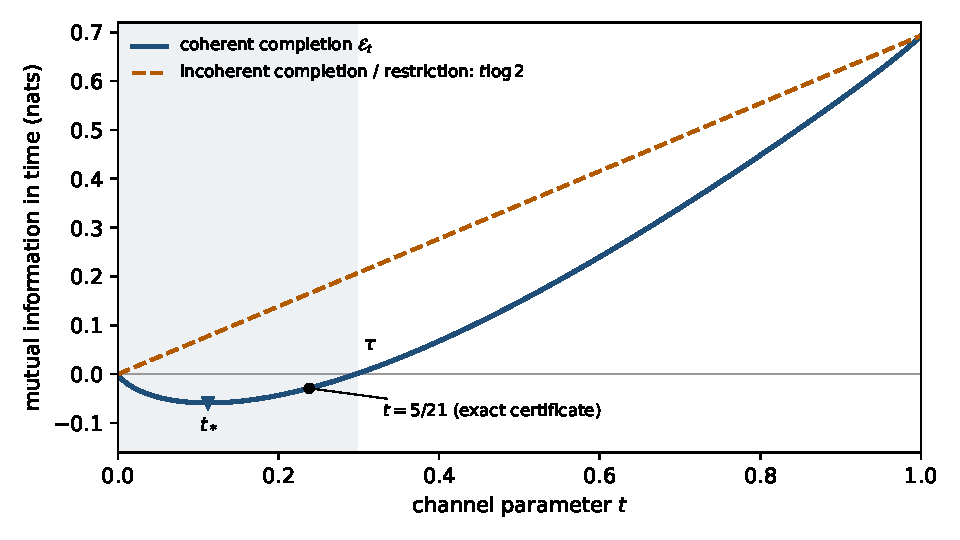
\includegraphics[width=0.92\linewidth]{qutrit_information.pdf}
\caption{Mutual information in time (nats) of the coherent erasure family $\E_t$ with $\rho=\diag(0,\tfrac12,\tfrac12)$ (solid), against the parameter $t$ of~\eqref{eq:k1}--\eqref{eq:channel}. It is negative on the shaded interval $(0,\tau)$, has its minimum at $t_*$, and reaches $\log2$ at $t=1$. The dot marks $t=5/21$, where the integer certificate~\eqref{eq:integer} applies. The dashed line, $t\log2$, is the common value of the incoherent completion and of the restricted qubit channel (Proposition~\ref{prop:support}).}
\label{fig:erasure}
\end{figure}

\section{A qutrit-to-qubit witness}\label{sec:qubitout}
The family of Section~\ref{sec:family} has output dimension three. This section shows that a qubit output suffices, so that the thresholds of Section~\ref{sec:lower} are attained simultaneously.

Define a linear map $\F:M_3(\mathbb C)\to M_2(\mathbb C)$ on matrix units by
\begin{equation}\label{eq:F}
\begin{aligned}
 &\F(\ket0\bra0)=\ket0\bra0,\qquad \F(\ket0\bra1)=c_1\ket0\bra1,\qquad \F(\ket0\bra2)=c_2\ket0\bra1,\\
 &\F(\ket1\bra1)=\diag(\alpha,1-\alpha),\qquad \F(\ket2\bra2)=\diag(\beta,1-\beta),\qquad \F(\ket1\bra2)=\gamma\,\diag(1,-1),
\end{aligned}
\end{equation}
and $\F(\ket j\bra i)=\F(\ket i\bra j)^*$, with the rational parameters
\[
 c_1=\tfrac{124}{125},\quad c_2=\tfrac1{47},\quad \alpha=\tfrac1{64},\quad \beta=\tfrac1{841},\quad \gamma=-\tfrac1{232},
 \qquad \rho_F=\diag\bigl(0,\tfrac1{47},\tfrac{46}{47}\bigr).
\]
As for $\E_t$, the unoccupied input level $\ket0$ is coupled coherently to the occupied ones, through $c_1$ and $c_2$; here $\ket0$ is sent to the output state $\ket0$.

\begin{theorem}\label{thm:qubitout}
$\F$ is a channel from $M_3(\mathbb C)$ to $M_2(\mathbb C)$, $\rho_F$ has rank two, and
\[
 I(\F,\rho_F)\in[-0.00139052762357144,\,-0.00139052762357143]\subset(-\infty,0).
\]
\end{theorem}
\begin{proof}
\emph{Channel.} Each $\F(\ket i\bra j)$ has trace $\delta_{ij}$, so $\F$ is trace preserving. In the ordering $\ket{ik}$ (input $i$, output $k$), the Choi matrix $C[\F]=\sum_{i,j}\ket i\bra j\otimes\F(\ket i\bra j)$ is the direct sum of the zero $1\times1$ block on $\ket{01}$, the block $\begin{psmallmatrix}\alpha&\gamma\\\gamma&\beta\end{psmallmatrix}$ on $\ket{10},\ket{20}$, and the block
$\begin{psmallmatrix}1&c_1&c_2\\c_1&1-\alpha&-\gamma\\c_2&-\gamma&1-\beta\end{psmallmatrix}$
on $\ket{00},\ket{11},\ket{21}$. The $2\times2$ block has determinant $\alpha\beta-\gamma^2=0$ and positive trace. The $3\times3$ block has leading principal minors $1$, $1-\alpha-c_1^2=\tfrac{311}{1000000}$ and determinant $\tfrac{329551}{11611056250}$, all positive. Hence $C[\F]\ge0$, and $\F$ is completely positive. (Equivalently, the characteristic polynomial of $C[\F]$ has coefficients of alternating sign.)

\emph{State over time.} Write $p=\tfrac1{47}$ and $q=\tfrac{46}{47}$. By Lemma~\ref{lem:blocks}, $\R_F=\R(\F,\rho_F)$ is the direct sum of the zero $1\times1$ block on $\ket{00}$, the block
\[
 B=\begin{pmatrix}p(1-\alpha)&-\gamma/2\\-\gamma/2&q(1-\beta)\end{pmatrix}\ \text{on }\ket{11},\ket{21},
\]
\[
 A=\begin{pmatrix}0&pc_1/2&qc_2/2\\pc_1/2&p\alpha&\gamma/2\\qc_2/2&\gamma/2&q\beta\end{pmatrix}\ \text{on }\ket{01},\ket{10},\ket{20}.
\]
Up to positive factors, their characteristic polynomials are
\begin{align*}
 &475588864\,x^2-474877284\,x+9735071 &&(B),\\
 &771516603548000000\,x^3-1154349536562500\,x^2\\
 &\qquad-172847845490527\,x+493204185796 &&(A).
\end{align*}
The quadratic has two positive roots and the cubic has one negative and two positive roots: approximately $-0.0155522$, $0.0029066$, $0.0141418$ (cubic) and $0.0209393$, $0.9775645$ (quadratic). The output state is $\F(\rho_F)=\diag(\tfrac{3785}{2529728},\tfrac{2525943}{2529728})$ and $S(\rho_F)=h(\tfrac1{47})$.

\emph{Certificate.} Each of the five nonzero roots was isolated exactly in an interval of rational endpoints of width below $10^{-45}$ (exact real-root isolation of the integer polynomials above, as implemented in SymPy), and $I(\F,\rho_F)$ was then evaluated in interval arithmetic at 60 significant digits from~\eqref{eq:entropy} and~\eqref{eq:mi}. The resulting enclosure is the displayed interval, whose upper end is negative.
\end{proof}

\begin{corollary}[All thresholds are attained at once]\label{cor:joint}
A process with $I(\E,\rho)<0$ has input dimension $d\ge3$, output dimension $m\ge2$ and initial rank at least $2$, and the process $(\F,\rho_F)$ has $d=3$, $m=2$ and rank $2$.
\end{corollary}
\begin{proof}
Combine Proposition~\ref{prop:FY} ($d\ge3$ and $m\ge2$), Proposition~\ref{prop:pure} (rank $\ge2$) and Theorem~\ref{thm:qubitout}.
\end{proof}
The violation of $\F$ is about forty times smaller than that of $\E_{t_*}$. Numerical searches over qutrit-to-qubit channels did not go below $-0.0013918$ (Section~\ref{sec:discussion}).

\section{Violations in the interior}\label{sec:interior}
Both witnesses so far sit on the boundary of the state space ($\rho$ has a zero eigenvalue), and $\E_t$ has a singular Choi matrix. This section shows that the violation survives small perturbations into the interior, so it is not a boundary artefact.

\begin{proposition}\label{prop:interior}
There are positive-definite qutrit states and qutrit channels with positive-definite Choi matrices for which $I(\E,\rho)<0$. One explicit choice is
\[
 \rho_\varepsilon=\diag(\varepsilon,(1-\varepsilon)/2,(1-\varepsilon)/2),
 \qquad
 \E_{t,\eta}=(1-\eta)\E_t+\eta\mathcal D,
\]
where $\mathcal D(X)=\Tr(X)\one_3/3$, $t=5/21$ and $\varepsilon=\eta=10^{-6}$. Every process close enough to this one also violates.
\end{proposition}
\begin{proof}
\emph{A modulus of continuity.} For $x,y\in[-1,1]$ with $|x-y|\le\delta\le1/e$,
\[
 \bigl|x\log|x|-y\log|y|\bigr|\le\omega(\delta):=\delta\log(2e/\delta).
\]
If $x,y$ have the same sign this is the standard estimate $|u\log u-v\log v|\le-\delta\log\delta\le\omega(\delta)$ for $u,v\in[0,1]$. If they have opposite signs then $|x|+|y|\le\delta$, and by concavity $-|x|\log|x|-|y|\log|y|\le\delta\log(2/\delta)\le\omega(\delta)$. For $N\times N$ Hermitian matrices $A,B$ with spectra in $[-1,1]$ and $\|A-B\|_\op\le\delta$, pairing the eigenvalues in increasing order and using Weyl's inequality gives
\begin{equation}\label{eq:continuity}
 |S(A)-S(B)|\le N\omega(\delta).
\end{equation}
The Fannes-type inequality of~\cite[Proposition~1]{FP} needs paired eigenvalues of equal sign, which we do not want to assume; hence this cruder modulus. States over time have spectra in $[-1,1]$, because $\|\J[\E]\|_\op\le1$ for every channel~\cite[Lemma~2.7]{FY}.

\emph{Perturbation sizes.} Write $\R=\R(\E_t,\rho)$ and $\R'=\R(\E_{t,\eta},\rho_\varepsilon)$. First, $\|\rho_\varepsilon-\rho\|_\op=\varepsilon$. Second,
$\E_{t,\eta}(\rho_\varepsilon)-\E_t(\rho)=\E_{t,\eta}(\rho_\varepsilon-\rho)+\eta(\mathcal D(\rho)-\E_t(\rho))$; a channel does not increase the trace norm, $\|\rho_\varepsilon-\rho\|_1=2\varepsilon$, and the difference of two states has operator norm at most $1$, so the operator norm is at most $2\varepsilon+\eta$. Third, $\J[\E_{t,\eta}]=(1-\eta)\J[\E_t]+\eta\one_9/3$, so
\[
 \R'-\R=\tfrac12\{(\rho_\varepsilon-\rho)\otimes\one,\J[\E_{t,\eta}]\}+\tfrac\eta2\{\rho\otimes\one,\one_9/3-\J[\E_t]\},
\]
and $\|\R'-\R\|_\op\le\varepsilon+\eta\|\rho\|_\op\cdot\tfrac43=\varepsilon+\tfrac{2\eta}3$. All three differences are at most $\delta=3\cdot10^{-6}$.

\emph{Conclusion.} The matrices in~\eqref{eq:mi} have sizes $3,3,9$, so by~\eqref{eq:continuity} $I$ changes by at most $15\,\omega(3\cdot10^{-6})$. Since $e>5/2$ and $(5/2)^{15}>2/(3\cdot10^{-6})$, we have $\log(2e/\delta)<16$, so $15\,\omega(\delta)<0.00072$. The integer comparison $3\cdot2573571875<8707129344$ strengthens~\eqref{eq:integer} to $I(5/21)<-\tfrac{\log3}{42}<-\tfrac1{42}$. Hence $I(\E_{t,\eta},\rho_\varepsilon)<-\tfrac1{42}+0.00072<0$. The state $\rho_\varepsilon$ is positive definite, and $C[\E_{t,\eta}]\ge\eta\one_9/3>0$. Continuity of $I$ gives an open neighbourhood of violating processes.
\end{proof}
The bound is deliberately crude; the actual perturbed value is $-0.0290183\ldots$, close to $I(5/21)=-0.0290202\ldots$.

\section{Coherent and incoherent completions}\label{sec:support}
Corollary~\ref{cor:rank2} says that coherence across the support is necessary for a rank-two violation. This section shows how much it matters: two channels that agree on the occupied subspace and on the unoccupied level give opposite signs.

Let $H=\operatorname{span}\{\ket1,\ket2\}$ and $U=\ket2\bra1-\ket1\bra2$. The restriction of $\E_t$ to operators supported on $H$ is the qubit erasure channel (followed by the rotation $U$)
\begin{equation}\label{eq:erasure}
 \mathcal F_t(X)=(1-t)\Tr(X)\ket0\bra0+tUXU^*,\qquad \mathcal F_t:M_2(\mathbb C)\to M_3(\mathbb C).
\end{equation}

\begin{proposition}\label{prop:support}
For the input $\one_2/2$ on $H$, $I(\mathcal F_t,\one_2/2)=t\log2\ge0$. The channel $\widetilde\E_t$ with the five Kraus operators
\[
 \tfrac1{\sqrt2}\ket1\bra0,\quad
 \tfrac1{\sqrt2}\ket2\bra0,\quad
 \sqrt{1-t}\,\ket0\bra1,\quad
 \sqrt{1-t}\,\ket0\bra2,\quad K_3(t)
\]
agrees with $\E_t$ on every $\ket i\bra j$ with $i,j\in H$ and on $\ket0\bra0$; the two channels differ only on the cross blocks $\ket i\bra0$, $\ket0\bra i$ ($i=1,2$). With the same input $\rho=\diag(0,\tfrac12,\tfrac12)$ and the same output state,
\[
 I(\widetilde\E_t,\rho)=t\log2\ge0,\qquad I(\E_t,\rho)<0\quad(0<t<\tau).
\]
\end{proposition}
\begin{proof}
By~\eqref{eq:blocks} with $\rho=\one_2/2$, the state over time of~\eqref{eq:erasure} has eigenvalues $(1-t)/2$ twice, $t/2$ three times and $-t/2$ once, so its entropy is $h(t)+\log2$. The marginal entropies are $\log2$ and $h(t)+t\log2$, which gives $t\log2$. The adjoint products of the five Kraus operators sum to $\one_3$, and a direct comparison of the images of matrix units gives the stated agreement and difference; in particular $\widetilde\E_t(\ket i\bra0)=0$ for $i=1,2$. Thus $\widetilde\E_t$ has no cross-coherence across $H$, and Proposition~\ref{prop:nocross} gives $I(\widetilde\E_t,\rho)=I(\mathcal F_t,\one_2/2)$. The coherent value is Theorem~\ref{thm:convex}.
\end{proof}

The state over time records how a channel acts on coherences between the initially occupied subspace and its complement, which are never populated in the process itself. Such data describe the process's response to interventions that prepare those coherences, not what happens when it runs on $\rho$. That $I$ is not invariant under restriction to the support is already implicit in~\cite{FP}: for a pure input the restricted channel has a one-dimensional input and mutual information $0$, whereas disturbing measurement processes with pure input have $I=-K>0$~\cite[Remark~4 and Theorem~2]{FP} (for instance, dephasing in the computational basis applied to $(\ket0-\ket1)/\sqrt2$ gives $I=\sqrt2\log(1+\sqrt2)-\log2>0$). What Proposition~\ref{prop:support} adds is a change of \emph{sign}: this unobserved part of the channel can decide whether the mutual information is negative. It does not claim that $\E_t$ and $\widetilde\E_t$ are indistinguishable: sequential measurements that create coherence between $H$ and $\ket0$ separate them.

\section{Discussion and open questions}\label{sec:discussion}
This section draws consequences, records numerical observations that are not used in any proof, and lists open questions.

\paragraph{Consequences.} (i) The subadditivity-based test proposed in~\cite{FP}, which declares an operator not to be a state over time when subadditivity fails, rejects genuine states over time. This happens already in the smallest possible dimensions (Corollary~\ref{cor:joint}) and on an open set of processes with full-rank state and positive-definite Choi matrix (Proposition~\ref{prop:interior}). (ii) Any non-negative information measure built from the same entropy needs a different construction or extra hypotheses. For rank-two states, Corollary~\ref{cor:rank2} identifies cross-coherence as the feature such hypotheses must control. (iii) The conjecture of~\cite{WPVF} that $0\le I\le1$ bit for a single qubit at two times concerns qubit inputs and is untouched; its lower half is~\cite[Theorem~4.1]{FY}.

\paragraph{Why random sampling missed the violations.} Fullwood and Parzygnat sampled random processes and found no violation~\cite[Section~5]{FP}. Violations appear to occupy a small region. In our reproducible experiment, $4000$ random qutrit processes with rank-two inputs and $1$ to $3$ Kraus operators gave no negative value. The violating examples found have a nearly rank-deficient input and a specifically coherent completion, which is where Corollary~\ref{cor:rank2} directs the search.

\paragraph{Numerical observations.} (a) Searches over complex qutrit channels and arbitrary qutrit states (25 random starts each with $3$ and with $9$ Kraus operators) reached at best $-0.0590860$, with $3$ Kraus operators. This is the family minimum $I(t_*)$; nothing lower was found. (b) Over qutrit-to-qubit channels, a structured search reached $-0.0013918$, slightly below the rational witness of Theorem~\ref{thm:qubitout}. (c) For tensor powers of the coherent erasure process at $t_*$,
\[
 I(\E_{t_*}^{\otimes k},\rho^{\otimes k})\approx-0.05909,\ -0.11912,\ -0.18016\qquad(k=1,2,3),
\]
slightly more negative than $kI(t_*)$. The anticommutator does not factor over tensor products, so additivity is not automatic. These values suggest that $I$ is unbounded below as the dimension grows.

\paragraph{Open questions.} Is $\inf I(\E,\rho)=-\infty$ over all finite dimensions, and how does the most negative value scale with $d$ and $m$? Is $I(t_*)$ the minimum over all qutrit processes, and what is the minimum over qutrit-to-qubit processes? Which qubit-input channels admit a violating coherent completion, and can the cross blocks of Lemma~\ref{lem:blocks} be turned into a necessary and sufficient criterion?

\section*{Verification and data availability}
The accompanying script \texttt{verify\_qutrit.py} (SymPy) builds every state over time directly from~\eqref{eq:definitions}, without using the claimed spectra. It checks the Kraus identities, both marginals, the characteristic polynomials of $\R_t$ at $t=5/21,7/40,11/96$, the integer certificate, the second-derivative formula~\eqref{eq:second} (to 40 digits at six sample points) and the rational identity in~\eqref{eq:convexlower}, the channel property and the certified interval of Theorem~\ref{thm:qubitout}, the constants of Proposition~\ref{prop:interior}, and the zero-padding identity behind Proposition~\ref{prop:support}. It exits with an error if any check fails, including under \texttt{python -O}. The script \texttt{numerics.py} (NumPy and SciPy, fixed seeds) reproduces the numerical observations of Section~\ref{sec:discussion}, which are not used in any proof. The proofs have not been formalised in a proof assistant.

\section*{AI-use statement}
This paper was prepared with substantial assistance from AI systems, which were used for the mathematical exploration, the proofs, the computations, the literature search and the drafting. Every computation reported here is reproducible with the accompanying scripts.

\begin{thebibliography}{9}
\bibitem{FP}
J. Fullwood and A. J. Parzygnat,
\emph{On dynamical measures of quantum information},
Entropy \textbf{27}(4) (2025), 331.
\url{https://doi.org/10.3390/e27040331}.

\bibitem{FY}
J. Fullwood and B. Yang,
\emph{On the entropy of a pseudo-density matrix},
arXiv:2608.28946v1 (2026).
\url{https://arxiv.org/abs/2608.28946}.

\bibitem{Omega}
The Omega Institute,
\emph{Subadditivity of the entropy of quantum states over time},
research dossier, release 8f61e708e239, with preregistration issue \#14994 of the repository
\url{https://github.com/the-omega-institute/trureturing}; accessed 15 November 2026.
\url{https://www.trureturing.org/research/fullwood-parzygnat-2025-states-over-time-subadditivity/}.

\bibitem{WPVF}
Z. Wu, A. J. Parzygnat, V. Vedral and J. Fullwood,
\emph{Quantum mutual information in time},
New J. Phys. \textbf{27}(6) (2025), 064504.
\url{https://doi.org/10.1088/1367-2630/adde7d}; arXiv:2410.02137.
\end{thebibliography}
\end{document}
